\documentclass[letter,12pt]{article}

\RequirePackage{amsmath}
\RequirePackage{amsmath,amssymb,amsthm}
\RequirePackage{tikz}
\usepackage{listings}
\usepackage{color}
\usepackage{textcomp}
\usepackage{graphicx}
\usepackage{hyperref}
\usepackage{afterpage}

\renewcommand{\lstlistlistingname}{Code Listings} 
\renewcommand{\lstlistingname}{Code Listing} 
\definecolor{gray}{gray}{0.5} 
\definecolor{key}{rgb}{0,0.5,0} 
\lstnewenvironment{python}[1][]{ 
\lstset{
language=python,
basicstyle=\ttfamily\small,
otherkeywords={1, 2, 3, 4, 5, 6, 7, 8 ,9 , 0, -, =, +, [, ], (, ), \{, \}, :, *, !},
keywordstyle=\color{blue},
stringstyle=\color{red},
showstringspaces=false,
emph={class, pass, in, for, while, if, is, elif, else, not, and, or,
def, print, exec, break, continue, return},
emphstyle=\color{black}\bfseries,
emph={[2]True, False, None, self},
emphstyle=[2]\color{key},
emph={[3]from, import, as},
emphstyle=[3]\color{blue},
upquote=true,
morecomment=[s]{"""}{"""},
commentstyle=\color{gray}\slshape,
frame=tb,
rulesepcolor=\color{blue},#1
}}{}


\usetikzlibrary{calc}
\RequirePackage{tkz-euclide}
\usetkzobj{all}

\setlength{\textheight}{8.5in}
\setlength{\headheight}{.25in}
\setlength{\headsep}{.25in}
\setlength{\topmargin}{0in}
\setlength{\textwidth}{6.75in}
\setlength{\oddsidemargin}{0in}
\setlength{\evensidemargin}{0in}


%%%%%%%%%%%%%%%%%%%%%%%%%%%%%%%%%%%%%%%%%%%%%%%%%%%%%%%%%%%%%%%%%%%%%%%
% Macros

% Math Macros.  It would be better to use the AMS LaTeX package,
% including the Bbb fonts, but I'm showing how to get by with the most
% primitive version of LaTeX.  I follow the naming convention to begin
% user-defined macro and variable names with the prefix "my" to make it
% easier to distiguish user-defined macros from LaTeX commands.
%
\newcommand{\myN}{\hbox{N\hspace*{-.9em}I\hspace*{.4em}}}
\newcommand{\myZ}{\hbox{Z}^+}
\newcommand{\myR}{\hbox{R}}

\newcommand{\myfunction}[3]
{${#1} : {#2} \rightarrow {#3}$ }

\newcommand{\myzrfunction}[1]
{\myfunction{#1}{{\myZ}}{{\myR}}}


% Formating Macros
%

\newcommand{\myheader}[4]
{\vspace*{-0.5in}
\noindent
{#1} \hfill {#3}

\noindent
{#2} \hfill {#4}

\noindent
\rule[8pt]{\textwidth}{1pt}

\vspace{1ex} 
}  % end \myheader 

\newcommand{\myalgsheader}[0]
{\myheader{Stanford University, Department of Computer Science}
{Computer Science 224n}{Spring 2017}{Section 1}}

% Running head (goes at top of each page, beginning with page 2.
% Must precede by \pagestyle{myheadings}.
\newcommand{\myrunninghead}[2]
{\markright{{\it {#1}, {#2}}}}

\newcommand{\myrunningalgshead}[2]
{\myrunninghead{Computer Science 224n}{{#1}}}

\newcommand{\myrunninghwhead}[2]
{\myrunningalgshead{Solution to Assignment {#1}, Problem {#2}}}

\newcommand{\mytitle}[1]
{\begin{center}
{\large {\bf {#1}}}
\end{center}}

\newcommand{\myhwtitle}[3]
{\begin{center}
{\large {\bf Solution to Assignment {#1}, Problem {#2}}}\\
\medskip
{\it {#3}} % Name goes here
\end{center}}

\newcommand{\myhwintro}[3]
{\begin{center}
{\large {\bf Assignment {#1}, Problem {#2}}}\\
\medskip
{\it {#3}} % Name goes here
\end{center}}

\newcommand{\mysection}[1]
{\noindent {\bf {#1}}}
\newcommand{\solutionsAuthor}{Akash Rana}
%%%%%% Begin document with header and title %%%%%%%%%%%%%%%%%%%%%%%%%
\begin{document}

\myalgsheader
\pagestyle{myheadings}
\thispagestyle{plain}
\setcounter{page}{1}
\myhwtitle{1}{1(a)}{\solutionsAuthor}

\bigskip


\noindent {\bf Softmax} Prove that $softmax$ is invariant to constant offsets in the input, that is, for any input vector $x$ and any constant $c$,
\begin{equation}
\textrm{softmax}({\bf x}) = \textrm{softmax}({\bf x }+ c),
\end{equation}
where $({\bf x} + c)$ means adding the constant $c$ to every dimension of ${\bf x}$.

\noindent\rule{\textwidth}{0.4pt}\vspace{5mm}

\begin{equation}
\textrm{softmax}({\bf x})_{j} = \frac{e^{x_{j}}}{\sum_{k=1} {e^{x_{k}}}}
\end{equation}
\ Solution:
\begin{align}
\textrm{softmax}({\bf x} + c)_{j} & = \frac{e^{(x_{j} + c)}}{\sum_{k=1}
			 {e^{(x_{k} + c)}}}\\
			& = \frac{e^{c}} {e^{c}} \frac{e^{(x_{j})}}{sum_{k=1} {e^{(x_{j})}}}\\
			& = \textrm{softmax}({\bf x})_{j}
\end{align}


\clearpage
\pagestyle{myheadings}
\myrunninghwhead{1}{1 (softmax)}

\myhwtitle{1}{1(b)}{\solutionsAuthor}
\bigskip

\noindent Given an input matrix of \texttt{N}-rows and \texttt{d}-columns, compute the softmax prediction for each row.
Write your implementation in \texttt{q1\_softmax.py}. You may test by executing python \texttt{q1\_softmax.py}.\\

\noindent \textbf{Note:} The provided tests are not exhaustive. Later parts of the assignment will reference this code so it is
important to have a correct implementation. Your implementation should also be efficient and vectorized
whenever possible. A non-vectorized implementation will not receive full credit!\vspace{5mm}

\noindent\rule{\textwidth}{0.4pt}

\begin{python}
import numpy as np

def softmax(x):
#x.shape by default gives column value
    if len(x.shape) > 1:
        # Matrix
        ### YOUR CODE HERE
        c = np.max(x, axis=1).reshape(-1,1) #-1 here means, internally  numpy is just calculating, to get the missing dimension.
        x = np.exp(x-c) / np.sum(np.exp(x-c), axis=1).reshape(-1,1)
        print (np.shape(x)) 
        ### END YOUR CODE
    else:
        # Vector
        ### YOUR CODE HERE
        c = np.max(x)
        x = np.exp(x-c) / np.sum(np.exp(x-c))
        ### END YOUR CODE

    assert x.shape == orig_shape
    return x
\end{python}

\clearpage 

\myrunninghwhead{1}{2 (Neural Networks)}

\myhwtitle{1}{2(a)}{\solutionsAuthor}

\bigskip

\noindent Derive the gradients of the sigmoid function and show that it can be rewritten as a function of the
function value (i.e. in some expression where only $\sigma(x)$, but not $x$, is present). Assume that the input
$x$ is a scalar for this question.\vspace{5mm}

\noindent\rule{\textwidth}{0.4pt}\vspace{5mm}

\noindent Denote the sigmoid function as $\sigma(z)$,
\begin{equation}
\sigma(z) = \frac{1}{1 + e^{-z}},
\end{equation}

Using chain rule, 

\begin{align*}
\sigma^{\prime}(z)   &= \frac{-1}{(1+e^{-z})^{2}}\times(-e^{-z})\\
                                 &= \(\frac{1}{1 + e^{-z}} \left(\frac{e^{-z}}{1 + e^{-z}} \right) \\
                                 &= \left(\frac{1}{1 + e^{-z}} \right) \left(\frac{1 + e^{-z}} {1 + e^{-z}} - \frac{1}{1 + e^{-z}} \right) \\
                                 &= \sigma(z)(1 - \sigma(z))
\end{align*}                                 

\clearpage

\myhwtitle{1}{2(b)}{\solutionsAuthor}
\bigskip

\noindent Derive the gradient with regard to the inputs of a softmax function when cross entropy loss is used for
evaluation, i.e. find the gradients with respect to the softmax input vector $\theta$, when the prediction is
made by $\hat{y} = \textrm{softmax}(\theta)$. Remember the cross entropy function is
\begin{equation}
\textrm{CE}({\bf y},{\bf\hat{y}}) = -\sum_{i}{y_{i}\log{\hat{y_{i}}}}
\end{equation}
where $y$ is the one-hot label vector, and $\hat{y}$ is the predicted probability vector for all classes. \vspace{2mm}\\
\noindent {\bf Hint}: you might want to consider the fact many elements of $y$ are zeros, and assume that only the $k$-th dimension
of $y$ is one.\vspace{5mm}

\noindent\rule{\textwidth}{0.4pt}\vspace{5mm}

Cross entropy error function for multi-class output,
\begin{equation}
\textrm{CE}({\bf y},{\bf\hat{y}}) = -\sum_{i}{y_{i}\log{\hat{y_{i}}}}
\end{equation}

Computing the gradient yields, 

\begin{equation}
\frac{\partial(\textrm{CE})}{\partial{\hat{y}_{i}}} = -\frac{y_{j}}{\hat{y}_i}\
\label{eq:2b 1}
\end{equation}


\begin{align}
\frac{\partial(\textrm{CE})}{\partial{\theta_{k}}} = & \frac{\partial(\textrm{CE})}{\partial{\hat{y}_{i}}}\frac{\partial{\hat{y}_{i}}}{\partial{\theta_{k}}} \\
                                                                        = & -\frac{y_{j}}{\hat{y}_{i}}\frac{\partial{\hat{y}_{i}}}{\partial{\theta_{k}}}
\end{align}

Calculating the partial derivative of $\hat{y_{i}}$ (derivation using the quotient rule):

\begin{align}
\text{if} \; i = k :& \frac{\partial y_i}{\partial \theta_i}= \frac{\partial  \frac{e^{\theta_i}}{\Sigma_\theta}}{\partial \theta_i} \\
												=& \frac{e^{\theta_i}\Sigma_\theta - e^{\theta_i}e^{\theta_i}}{\Sigma_\theta^2} \\
												=&\frac{e^{\theta_i}}{\Sigma_\theta}\frac{\Sigma_\theta - e^{\theta_i}}{\Sigma_\theta} \\
												=& \frac{e^{\theta_i}}{\Sigma_\theta}(1-\frac{e^{\theta_i}}{\Sigma_\theta}) =  \hat{y_i} (1 - \hat{y_i}) \label{eq:2b 2}
\end{align}
\begin{align}
												\text{if} \; i \neq k :& \frac{\partial y_i}{\partial \theta_j} =\frac{\partial \frac{e^{\theta_i}}{\Sigma_\theta}}{\partial \theta_j}\\
												= &\frac{0 - e^{\theta_i}e^{\theta_j}}{\Sigma_\theta^2} \\
												=& -\frac{e^{\theta_i}}{\Sigma_\theta} \frac{e^{\theta_j}}{\Sigma_\theta} \\
												=& -\hat{y_i} y_k \label{eq:2b 3}
\end{align}

Combining Equations~\ref{eq:2b 1},~\ref{eq:2b 2},~\ref{eq:2b 3}, yields
\begin{equation}
\frac{\partial(\textrm{CE})}{\partial{\theta_{k}}} = \begin{cases}
-y_{j}(1 - \hat{y}_{k})&\text{ for }i=k \\
y_{j}\hat{y}_{k}&\text{ for }i\neq k
\end{cases}
\end{equation}
Requiring $y_{j}$ to be non-zero, imposes that the auxiliary condition, $k=j$ and $y_{j}=1$, hence it follows immediately,
\begin{equation}
\frac{\partial(\textrm{CE})}{\partial{\theta_{j}}} = \begin{cases}
(\hat{y}_{j} - 1)&\text{ for }i=j\label{eq:2b case 1} \\
\hat{y}_{j}&\text{ for }i\neq j
\end{cases}
\end{equation}
Which is equivalent to
\begin{equation}
\frac{\partial(\textrm{CE})}{\partial{\boldsymbol\theta}} = \bf{\hat{y}} - \bf{y}
\end{equation}

\clearpage

\myhwtitle{1}{2(c)}{\solutionsAuthor}
\bigskip

\noindent Derive the gradients with respect to the inputs x to an one-hidden-layer neural network (that is, find
$\partial{J}/\partial{\bf x}$ where $J$ is the cost function for the neural network). The neural network employs sigmoid activation
function for the hidden layer, and softmax for the output layer. Assume the one-hot label vector is $y$,
and cross entropy cost is used. (feel free to use $\sigma^{\prime}(x)$ as the shorthand for sigmoid gradient, and feel free
to define any variables whenever you see fit). \vspace{5mm}\\

\noindent\rule{\textwidth}{0.4pt}\vspace{5mm}
In order to simplify the notation used to solve the problem, define the following terms:
\begin{align}
{\bf x}^{(2)} \equiv & \quad{\bf h} \\
{\bf z}_{i}     \equiv& \quad{\bf x^{(i)}\textrm{W}_{i} + b_{i}}
\end{align}
Now, to calculate $\partial{J}/\partial{\bf x^{1}}$, one can use the back propagation algorithm. Starting with the chain rule and then results from Question 2(b):

\begin{equation}
\frac{\partial{J}}{\partial{\bf x}^{(2)}}  = \left( \left(\frac{\partial{J}}{\partial{\bf z}_{2}}  \frac{\partial{\bf z}_{2}}{\partial{\bf x}^{(2)}}\right) . \frac{\partial{\bf x}^{(2)}}{\partial{\bf z}_{1}} \right) * \frac{\partial{\bf z}_{1}}{\partial{\bf x}^{(1)}}
\end{equation}

\begin{equation}
\frac{\partial{J}}{\partial{\bf z}_{2}} = \bf{\hat{y}} - \bf{y}
\end{equation}
and
\begin{equation}
\frac{\partial{\bf z}_{i}}{\partial{{\bf x}^{(i)}}} = {\bf \textrm{W}^{\top}_{i}}\label{eq: 2c 1}
\end{equation}
Sigmoid ($\sigma$) derivative can be found in Question 2(a), but we define:
\begin{equation}
\frac{\partial{{\bf x}^{(2)}}}{\partial{{\bf z}_{1}}}\equiv\sigma^{\prime}(z_{1})%{\bf x}^{(2)}\cdot(1  - {\bf x}^{(2)})
\end{equation}
Combining these, and using $\cdot$ to denote element-wise product:
\begin{equation}
\frac{\partial{J}}{\partial{z_{i}}} = (\bf{\hat{y}} - \bf{y}){\bf \textrm{W}^{\top}_{2}}\cdot\sigma^{\prime}(z_{1})
\end{equation}
Finally, using the results from Equation~\ref{eq: 2c 1} (but for the first layer):
\begin{equation}
\frac{\partial{J}}{\partial{{\bf x}^{(1)}}} = (\bf{\hat{y}} - \bf{y}){\bf \textrm{W}^{\top}_{2}}\cdot\sigma^{\prime}(z_{1})\cdot{\bf \textrm{W}^{\top}_{1}}
\end{equation}

\clearpage

\myhwtitle{1}{2(d)}{\solutionsAuthor}
\bigskip
\noindent How many parameters are there in this neural network, assuming the input is $\textrm{D}_{x}$-dimensional,
the output is $\textrm{D}_{y}$-dimensional, and there are H hidden units?\vspace{5mm}

\noindent\rule{\textwidth}{0.4pt}

\noindent $\bf{\textrm{W}}_{1}$ must have dimensions:  $\textrm{D}_{x}\times\textrm{H}$. The bias ($\bf{b}_{1}$) for the first layer must have
dimensions $\textrm{H}$. Adding these two together, yields $(\textrm{D}_{x} + 1)\times\textrm{H}$. Proceeding to the second layer,
there must be $\textrm{H}\times\textrm{D}_{y}$ parameters associated with the weight matrix ${\bf\textrm{W}}_{2}$. The bias ($\bf{b}_{2}$)
for the second layer must have dimensions $\textrm{D}_{y}$ elements. This yields, 
\begin{equation}
(\textrm{D}_{x} + 1)\times\textrm{H} + \textrm{D}_{y}\times(\textrm{H}+1)
\end{equation}
weights, for each input vector of dimensions $\textrm{D}_{x}$.

\clearpage

\myrunninghwhead{1}{3 (word2vec)}

\myhwtitle{1}{3(a)}{\solutionsAuthor}
\bigskip
\noindent Assume you are given a predicted word vector ${\boldsymbol v}_{c}$ corresponding to the center word $c$ for
\texttt{skipgram}, and word prediction is made with the \texttt{softmax} function found in \texttt{word2vec} models
\begin{equation}
{\hat{\boldsymbol y}}_{\boldsymbol o} = p(~{\boldsymbol o} \mid {\boldsymbol c}~) = \frac{\exp{({\boldsymbol u}^{\top}_{o}{\boldsymbol v}_{c})}}{\sum^{\vert{W}\vert}_{j=1}\exp{({\boldsymbol u}^{\top}_{j}{\boldsymbol v}_{c})}}
\end{equation}
where $w$ denotes the $w$-th word and ${\boldsymbol u}_{w}$ ($w=1,...,\vert\textrm{W}\vert$)  are the `output' word vectors for all words in the vocabulary ($v^{\prime}_{w}$ in the lecture notes). Assume the cross entropy cost is applied to this prediction and word $o$ is the expected word (the $o$-th element of the one-hot label vector is one), derive the gradients with respect to ${\boldsymbol v}_{c}$.\\

\noindent \textbf{Hint:} It will be helpful to use notation from question 2. For instance, letting ${\hat{\boldsymbol y}}$ be the vector of the softmax
prediction for every word, ${\boldsymbol y}$ as the expected word vector, and the loss function

\begin{equation}
J_{\textrm{softmax-CE}}({\boldsymbol o}, {\boldsymbol v}_{c}, {\boldsymbol U}) = CE({\boldsymbol y},{\hat{\boldsymbol y}})
\end{equation}
where ${\boldsymbol U} = [ {\boldsymbol u}_{1}, {\boldsymbol u}_{2},...,{\boldsymbol u}_{\vert\textrm{W}\vert}]$ is the matrix of all the output vectors. \textit{Make sure you state the orientation of your vectors and matrices.}\vspace{5mm}

Applying cross-entropy cost to the above softmax probability defined above:
\begin{equation}
J =-\log{p} = - {\boldsymbol u}_{o}^{\top}{\boldsymbol v}_{c} + \log\sum^{\vert{V}\vert}_{j=1}\exp{({\boldsymbol u}_{j}^{\top}{\boldsymbol v}_{c})}
\end{equation}
Let $z_{j}={\boldsymbol u}_{j}^{\top}{\boldsymbol v}_{c}$, and $\delta^{i}_{j}$ be the indicator function, then
\begin{equation}
\frac{\partial J}{\partial{z_{k}}} = - \delta^{i}_{k} + \frac{\exp{({\boldsymbol u}_{i}^{\top}{\boldsymbol v}_{c})}}{\sum^{\vert{V}\vert}_{j=1}\exp{({\boldsymbol u}_{j}^{\top}{\boldsymbol v}_{c})}}
\end{equation}
Now, using the chain rule, we can calculate,
\begin{align}
\frac{\partial J}{\partial{{\boldsymbol v}_{c}}} =& \frac{\partial J}{\partial{{\boldsymbol z}}}\frac{\partial{{\boldsymbol z}}}{\partial{{\boldsymbol v}_{c}}} \\
                                                                    =& \sum^{\vert{V}\vert}_{j=1}{\boldsymbol u}_{j}^{\top}\left(\frac{e^{z_{j}}}{\sum^{\vert{V}\vert}_{k=1}e^{z_{k}}} -  1\right) \\
                                                                    =& \sum^{\vert{V}\vert}_{k=1}{\boldsymbol P}({\boldsymbol u}_{j} \vert {\boldsymbol v}_{c} ){\boldsymbol u}_{j} - {\boldsymbol u}_{j}
\end{align}
\clearpage

\myhwtitle{1}{3(b)}{\solutionsAuthor}

\bigskip
\noindent As in the previous problem, derive gradients for the `output' word vectors ${\boldsymbol u}_{w}$'s (including ${\boldsymbol u}_{o}$)\vspace{5mm}
%TODO
%\hat{\boldsymbol r} -> {\boldsymbol v}_{c}
% {\boldsymbol w}^{\top}_{i} -> {\boldsymbol u}^{\top}_{0}
% (in sum) {\boldsymbol w}^{\top}_{k} -> {\boldsymbol u}^{\top}_{k}
% {\boldsymbol w}_{j} -> {\boldsymbol u}_{j}
\noindent\rule{\textwidth}{0.4pt}\vspace{5mm}
This follows immediately from the chain rule:
\begin{align}
\frac{\partial J}{\partial{\boldsymbol u}_{j}} = &\frac{\partial J}{\partial{{\boldsymbol z}}}\frac{\partial{{\boldsymbol z}}}{\partial{\boldsymbol u}_{j}} \\
                                                                  = &{\boldsymbol v}_{c}\left(\frac{\exp{({\boldsymbol u}^{\top}_{0}{\boldsymbol v}_{c})}}{\sum^{\vert{V}\vert}_{j=1}\exp{({\boldsymbol u}^{\top}_{j}{\boldsymbol v}_{c})}} - \delta^{0}_{j}\right)
\end{align}
\clearpage

\myhwtitle{1}{3(c)}{\solutionsAuthor}
\bigskip
%TODO
%\hat{\boldsymbol r} -> {\boldsymbol v}_{c}
% {\boldsymbol w}^{\top}_{i} -> {\boldsymbol u}^{\top}_{0}
% (in sum) {\boldsymbol w}^{\top}_{k} -> {\boldsymbol u}^{\top}_{k}
\noindent Repeat part (a) and (b) assuming we are using the negative sampling loss for the predicted vector ${\boldsymbol v}_{c}$, and 
the expected output word is ${\boldsymbol o}({\boldsymbol u}_{o})$. Assume that $K$ negative samples (words) are drawn, and they are ${\boldsymbol u}_{1},...,{\boldsymbol u}_{k}$, respectively for simplicity of notation ($k\in\{1,...,K\}$ and $o\notin\{1,...,K\}$). Again for a given word, ${\boldsymbol o}$, denote its output vector as ${\boldsymbol u}_{o}$. The negative sampling loss function in this case is,
\begin{equation}
J({\boldsymbol u}_{o}, {\boldsymbol v}_{c}, {\boldsymbol U}) = -\log(\sigma( {\boldsymbol u}^{\top}_{o}{\boldsymbol v}_{c})) - \sum^{K}_{k=1}\log(\sigma(- {\boldsymbol u}^{\top}_{k}{\boldsymbol v}_{c}))
\end{equation}
where $\sigma(\cdot)$ is the sigmoid function.\\

\noindent After you've done this, describe with one sentence why this cost function is much more efficient to
compute than the softmax-CE loss (you could provide a speed-up ratio, i.e. the runtime of the softmax-CE loss divided by the
runtime of the negative sampling loss).\\

\noindent {\bf Note}: the cost function here is the negative of what Mikolov \textit{et. al.} had in their original paper,
because we are doing a minimization instead of maximization in our code.\vspace{5mm}

\noindent\rule{\textwidth}{0.4pt}\vspace{5mm}


\begin{align}
\frac{\partial J}{\partial{\boldsymbol v}_{c}} = &\frac{\partial J}{\partial{{\boldsymbol p}_{i}}}\frac{\partial{{\boldsymbol p}_{i}}}{\partial{\boldsymbol x}_{j}}\frac{\partial{{\boldsymbol x}_{i}}}{\partial{\boldsymbol v}_{c}} + \sum^{{K}}_{k=1}\frac{\partial J}{\partial{{\boldsymbol p}_{i}}}\frac{\partial{{\boldsymbol p}_{i}}}{\partial{\boldsymbol z}_{k}}\frac{\partial{{\boldsymbol z}_{k}}}{\partial{\boldsymbol v}_{c}} \\
=&-(\bf{1- \bf{p}_{i}}){\bf \textrm{U}_{i}} + \sum^{{K}}_{k=1}(\bf{1- \bf{q}_{k}}){\bf \textrm{U}_{k}}                                                              
\end{align}

\begin{align}
\frac{\partial J}{\partial{\boldsymbol u}_{j}} = &\frac{\partial J}{\partial{{\boldsymbol p}_{i}}}\frac{\partial{{\boldsymbol p}_{i}}}{\partial{\boldsymbol x}_{j}}\frac{\partial{{\boldsymbol x}_{i}}}{\partial{\boldsymbol u}_{j}} + \sum^{{K}}_{k=1}\frac{\partial J}{\partial{{\boldsymbol p}_{i}}}\frac{\partial{{\boldsymbol p}_{i}}}{\partial{\boldsymbol z}_{k}}\frac{\partial{{\boldsymbol z}_{k}}}{\partial{\boldsymbol u}_{j}}\\
= &-(\bf{1- \bf{p}_{i}}){\bf \delta_{ij} \textrm{V}_{c}} + \sum^{{K}}_{k=1}(\bf{1- \bf{q}_{k}}){\bf\delta_{ij} \textrm{V}_{c}}                                                              
\end{align}
                    
where, $\delta_{xy}$ = kronecker delta \\
when $ {x = y} $ = 1 \\
0 , otherwise. 


\clearpage
\myhwtitle{1}{3(d)}{\solutionsAuthor}
%TODO FIX this 
\bigskip
\noindent Derive the gradients for all of the word vectors for \texttt{skip-gram} and \texttt{CBOW} (optional)
given a set of context words [$\texttt{word}_{c-\textbf{m}},...,\texttt{word}_{c-\textbf{1}},\texttt{word}_{c},\texttt{word}_{c+\textbf{1}},...,\texttt{word}_{c+\textbf{m}}$ ], where \textbf{m} is the context size. You can denote 
the `input' and `output' word vectors for $\texttt{word}_{k}$ as ${\boldsymbol v}_{k}$ and ${\boldsymbol u}_{k}$ respectively for
convenience. \\

\noindent {\bf Hint}: feel free to use $F({\boldsymbol o}, {\boldsymbol v}_{c})$ (where ${\boldsymbol o}$ is the expected word) as a placeholder for $J_{\texttt{softmax-CE}}({\boldsymbol o}, {\boldsymbol v}_{c}, ...)$ or $J_{\texttt{neg-sampling}}({\boldsymbol o}, {\boldsymbol v}_{c}, ...)$ cost functions in this part --- you'll see that this is a useful abstraction for the coding part. That is, your solution may contain terms of the form $\frac{\partial{F_{i}({\boldsymbol o}, {\boldsymbol v}_{c})}}{\partial\lambda}$.\\

\noindent Recall that for \texttt{skip-gram}, the cost for a context centered around $c$ is
\begin{equation}
J_{\texttt{skip-gram}} =   \sum_{-m\le j\le m, j\neq0}F({\boldsymbol w}_{c+j}, {\boldsymbol v}_{c})
\end{equation}
where ${\boldsymbol w}_{c+j}$ refers to the word at the $j$-th index from the center.\\

\noindent \texttt{CBOW} is slighltly different. Instead of using ${\boldsymbol v}_{c}$ as the prediction vector, we use $\hat{\boldsymbol v}$ defined below. For (a simpler variant of) \texttt{CBOW}, we sum up the input word vectors in the context:\\
\begin{equation}
\hat{\boldsymbol v} = \sum_{-m\le j\le m, j\neq0}{\boldsymbol v}_{c+j}
\end{equation}
then the \texttt{CBOW} cost is 
\begin{equation}
J_{\texttt{CBOW}}(\texttt{word}_{c-\textbf{m}} ,...,\texttt{word}_{c+\textbf{m}}) = F({\boldsymbol w}_{c}, \hat{\boldsymbol v})
\end{equation}
\noindent\textbf{Note}: To be consistent with the $\hat{\boldsymbol v}$ notation such as for the code portion, for \texttt{skip-gram} $\hat{\boldsymbol v} = {\boldsymbol v_{c}}$

\vspace{5mm}
\noindent\rule{\textwidth}{0.4pt}\vspace{5mm}



\noindent For skip-gram:
\begin{equation}
\frac {\partial {J_{\texttt{skip-gram}}}} {\partial U}  =   \sum_{-m\le j\le m, j\neq0}\frac {\partial{ F({\boldsymbol w}_{c+j}, {\boldsymbol v}_{c})}}{\partial {U}} 
\end{equation}

\begin{equation}
\frac {\partial {J_{\texttt{skip-gram}}}} {\partial v_{c}}  =   \sum_{-m\le j\le m, j\neq0}\frac {\partial{ F({\boldsymbol w}_{c+j}, {\boldsymbol v}_{c})}}{\partial {v}_{c}} 
\end{equation}

\begin{equation}
\frac {\partial {J_{\texttt{skip-gram}}}} {\partial v_{i}}  =  0 , For i \neq c
\end{equation}




\noindent For CBOW:

\begin{equation}
\frac {\partial {J_{\texttt{CBOW}}}} {\partial U}  = \frac {\partial{ F({\boldsymbol w}_{c}, {\boldsymbol {\hat{v}}})}} {\partial {U}} 
\end{equation}

\begin{equation}
\frac {\partial {J_{\texttt{CBOW}}}} {\partial {v}_{j}}  = \frac {\partial{ F({\boldsymbol w}_{c}, {\boldsymbol {\hat{v}}})}} {\partial {v}} 
\end{equation}

\begin{equation}
\frac {\partial {J_{\texttt{CBOW}}}} {\partial v_{j}}  =  0 , For i \neq c
\end{equation}
\clearpage

\myhwtitle{1}{4(b)}{\solutionsAuthor}
\bigskip
\noindent Explain in fewer than three sentences why we want to introduce regularization when doing classification (in fact, most machine learning tasks).\vspace{5mm}

\noindent\rule{\textwidth}{0.4pt}\vspace{5mm}
Regularization helps prevent over-fitting of training dataset. Simply put it helps to avoid model from memorizing the dataset and instead help to learn features well. 
\clearpage



\myhwtitle{1}{4(d)}{\solutionsAuthor}

\bigskip
\noindent Fill in the hyperparameter selection code in \texttt{q4\_sentiment.py} to search for the `optimal' regularization parameter. \textbf{What values did you select? Report your train, dev, and test accuracies. Justify your hyperparameter search methodology in at most one sentence.}. \\

\noindent\textbf{Note:} you should be able to attain at least 30\% accuracy on dev.\vspace{5mm}

\noindent\rule{\textwidth}{0.4pt}\vspace{5mm}

\begin{table}[!h!p]
\begin{center}
\begin{tabular}{c c c c}
\hline\hline


Reg   &  Train &  Dev & Test \\
\hline
1.00E-06 & 30.993 & 32.516 & 30.407 \\
1.00E-05 & 31.051 & 32.516  & 30.362 \\
1.00E-04 & 30.993 & 32.698  & 30.362 \\
1.00E-03 & 31.156 & 32.698  & 30.271 \\
1.00E-02 & 30.946 & 32.334  & 29.910 \\
1.00E-01 & 30.290 & 31.880  & 29.819 \\
1.00E+00 & 28.897 & 29.609  & 27.149 \\
1.00E+01 & 27.247 & 25.522  & 23.077 \\
1.00E+02 & 27.247 & 25.522  & 23.032 \\
1.00E+03 & 27.247 & 25.522  & 23.032 \\
1.00E+04 & 27.247 & 25.522  & 23.032 \\
1.00E+05 & 27.247 & 25.522  & 23.032 \\

\hline\hline
\end{tabular}
\end{center}
\end{table}

\begin{itemize}
\item The word vectors are trained on massive data (wikipedia), thus hold more
    information
\item GloVe represents words better than word2vec.
\item GloVe is a "count-based" model, they learn their vectors by essentially doing dimensionality reduction on the co-occurrence counts matrix.
\end{itemize}

\clearpage

\myhwtitle{1}{4(e)}{\solutionsAuthor}

\bigskip
\noindent Plot the classification accuracy on the train and dev set with respect to the regularization value, using a logarithmic scale on the x-axis. This should have been done automatically. \textbf{Include \texttt{q4\_reg\_acc.png} in your homework write up.} Briefly explain in at most three sentences what you see in the plot.\vspace{5mm}

\noindent\rule{\textwidth}{0.4pt}\vspace{5mm}

\begin{figure}[!h!p]
\begin{center}
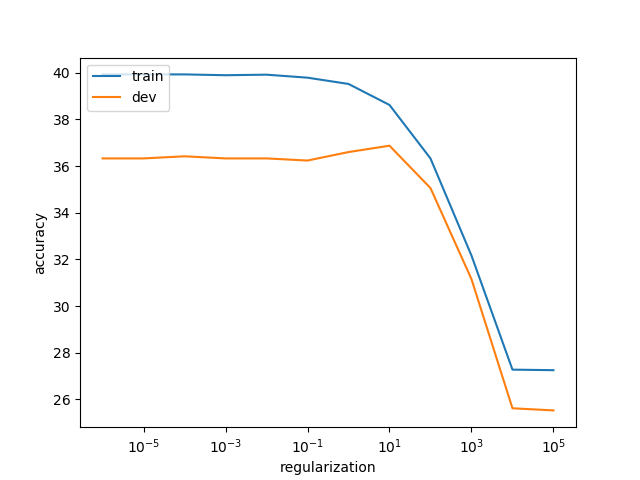
\includegraphics[scale=0.5]{../q4_reg_v_acc.png}
\end{center}
Regulariztion helps avoiding overfitting of the model.
As we increase regularization parameter the model losses its accuracy.
\end{figure}


\clearpage

\myhwtitle{1}{4(f)}{\solutionsAuthor}


\bigskip
\noindent We will now analyze errors that the model makes (with pretrained GloVe vectors). When you ran python q4 sentiment.py --pretrained, two files should have been generated. Take a look at q4 dev conf.png and include it in your homework writeup. Interpret the confusion matrix in at most three sentences.
\begin{figure}[!h!p]
\begin{center}
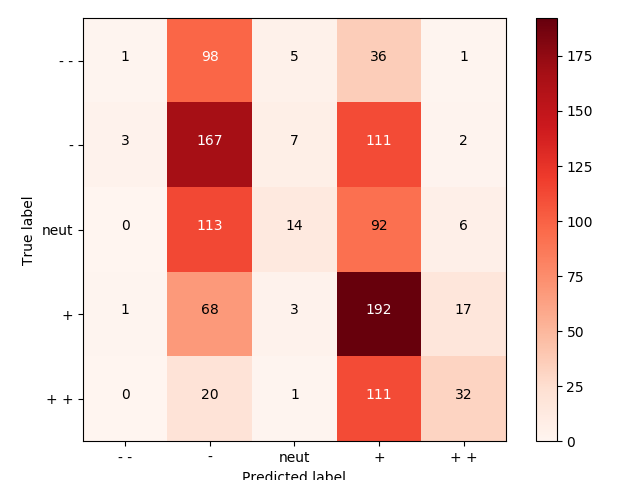
\includegraphics[scale=0.5]{../q4_dev_conf.png}
\end{center}
The prediction for extremums looks pretty coreect.  
 Whereas for negative, neturals and positive examples the model misjudged.
 Overall the quality looks decent.
\end{figure}

\clearpage

\myhwtitle{1}{4(g)}{\solutionsAuthor}


\bigskip
\noindent Next, take a look at q4 dev pred.txt. Choose 3 examples where your classifier made errors
and briefly explain the error and what features the classifier would need to classify the example correctly
(1 sentence per example). Try to pick examples with different reasons.

\begin{enumerate}

\item Some cold/negative words in the sentence cause the whole sentence to be predicted as negative, while the sentence has a positive context.
True   Predicted
\begin{itemize}

 \item ++   -   this flick is about as cool and crowd-pleasing as a documentary can get 
\end{itemize}
\item Some negative words doesn't contribute to the sentiment or they are countered as double negatives
\begin{itemize}
\item -   +   an absurdist comedy about alienation , separation and loss .
\end{itemize}

\item The positive words are given more importance then overall meaning of sentence.
\begin{itemize}

\item 0   ++   a beautifully made piece of unwatchable drivel
\end{itemize}

\end{enumerate}


\end{document}